% ================= SISTEMI LINEARI ==================================================

\section{Sistemi Lineari}

\subsection{Equazioni Lineari}

\centering\( x_1 - 2x_2 = 3\) \textsf{\small è un'equazione lineare  nelle incognite $x_1, x_2$} \\
\( x_1^2 - 3x_2 = 0\) \textsf{\small \underline{NON} è lineare.}
\vspace{-5mm} %\hfill
\subsection{Sistemi Lineari}
%\vspace{-2mm}
\textsf{\small E' un insieme di $n$ equazioni lineari che devono essere soddisfatte.}

\noindent\begin{minipage}{.2\linewidth}
\(
\begin{cases*}
x_1 - x_2 = 0 \\
x_2 = 1
\end{cases*}
\)
\end{minipage}
\begin{minipage}{.2\linewidth}
\(
\Rightarrow x_1 = x_2 = 1
\)
\end{minipage}

\textsf{\small Si dicono EQUIVALENTI se hanno esattamente lo stesso insieme di soluzioni.}
\vspace{-3mm}
\subsection{Matrici}

\( m, n \in \mathbb{N} = {1, 2, 3, \cdots}\)
\textsf{\small \textcolor{red}{m} righe e \textcolor{blue}{n} colonne.}

\[
A = 
\begin{pmatrix}
	1 & \overset{\text{posizione:} 1,2}{2} & 3 \\
	4 & 5 & 6 
\end{pmatrix}
\]

\subsubsection{Moltiplicazione tra matrici}

\textsf{\small Righe per colonne.}
\begin{comment}
\begin{align}
	P^+ &= \begin{pmatrix}
		1 & 0 \\
		0 & 0
	\end{pmatrix}
	&
	P^- &= \begin{pmatrix}
		0 & 0 \\
		0 & 1
	\end{pmatrix}
\end{align}
\end{comment}

\[
\begin{pmatrix}
\tikzmark{starta}1 & -1 & 0\tikzmark{enda} \\
2 & 0 & \frac{1}{2}
\end{pmatrix}
\begin{pmatrix}
1 \\ 2 \\ -2
\end{pmatrix}
=
\begin{pmatrix}
1 - 2 + 0 \\
2 + 0 - 1 
\end{pmatrix}
=
\begin{pmatrix}
-1 \\
1
\end{pmatrix}
\]

\begin{tikzpicture}[remember picture,overlay]
	\foreach \Val in {a}
	{
		\draw[rounded corners,red,thick]
		([shift={(-0.5\tabcolsep,-0.5ex)}]pic cs:start\Val) 
		rectangle 
		([shift={(0.5\tabcolsep,2ex)}]pic cs:end\Val);
	}
\end{tikzpicture}

\begin{tikzpicture}[overlay]
	\draw[red, line width=.5pt] (1.35,1.7) ellipse (0.2cm and .9cm);
\end{tikzpicture}
{\bf Sistemi Lineari e Matrici} \\
\textsf{\small Riscriviamo ogni sistema lineare in termini di matrici.}

\(
\begin{cases*}
x_1 - 2x_2 + 3x_3 = 1 \\
2x_1 - x_2 - x_3 = 2
\end{cases*}
\)

\enlargethispage{5\linewidth}
\[
A =
\underbrace{
\begin{pmatrix}
	1 & -2 & 3\\
	2 & -1 & -1
\end{pmatrix}
} _{\text{Matrice Incompleta}}
\begin{pmatrix}
	x_1 \\ x_2 \\ x_3
\end{pmatrix}
=
\begin{pmatrix}
	1 \\
	2
\end{pmatrix}
\]

\[
\underbrace{
\left(
\begin{matrix}
1 & -2 & 3 \\
2 & -1 & -1
\end{matrix}
\middle\vert
\begin{matrix}
1 \\ 2
\end{matrix}
\right)
} _{\text{Matrice Completa}}
\]

\begin{comment}
\begin{equation*}
\left(
%
\begin{array}{l}
	\alpha_T     \\
	\alpha_{T-1}
\end{array}
%
\middle\vert
%
\;y_{1:T-1},\,\boldsymbol{\theta}
%
\right)
\end{equation*}
\end{comment}

% ================= MATRICE QUADRATA =========================================

\newpage

\subsubsection{Matrice Quadrata}

\textsf{\small Se m = n (ovvero numero di righe = numero di colonne) la matrice è QUADRATA di ordine n.} \\

%\textbf{\textcolor{red}{A SCALA}} \\

\textsf{\small Una matrice m $\cdot$ n si dice a scala (per righe) se soddisfa le seguenti proprietà: } \\

\begin{enumerate}
	\item \textsf{\small Eventuali righe nulle (che contengono solo 0) si trovano in fondo alla matrice}
	\item \textsf{\small Il primo elemento non nullo di ogni riga (non nulla) si trova più a destra del primo elemento non nullo della riga precedente}
\end{enumerate}

\(
A =
	\begin{pmatrix}
		1 & 0 & -3 & 2\\
		0 & 1 & 3 & 3 \\
		0 & 0 & 0 & 0
	\end{pmatrix}
\)
\( \text{rg}(A) = 2\)

%\begin{comment}
\[
\begin{tikzpicture}[remember picture,overlay]
	\draw[red] (-1.8, 2) -- (-1.2,2) -- (-1.2, 1.5);
	\draw[red] (-1.2,1.5) -- (-0.5,1.5) -- (-0.5, 0.8);
	\draw[red] (-0.5, 0.8) -- (0.6, 0.8);
\end{tikzpicture}
\]
%\end{comment}

%\textbf{\textcolor{red}{RANGO}}
\subsubsection{RANGO}

\textsf{\small Data una matrice a scala A si dice rango di A e si indica rg(A) il numero di righe non nulle di A.} \\
\textsf{\small \textcolor{red}{\underline{Attenzione:}} Questa definizione di rango vale solo per le matrici a scala.}

\textsf{\small \textcolor{ForestGreen}{Terminologia: } in una matrice a scala il primo elemento non nullo di ogni riga si chiama PIVOT} \\
$\implies$\textsf{\small il rango di una matrice a scala è il numero di pivot della matrice. }

\textsf{\small \textcolor{red}{risolvo per sostituzioni successive dal basso}} \\
\begin{minipage}{.3\linewidth}
\(
\begin{cases*}
	x_1 - x_2 = 1\\
	x_2 - 3x_3 = 2\\
	-x_3 = 1
\end{cases*}
\)
\end{minipage}
\begin{minipage}{.3\linewidth}
\(
\begin{cases*}
	x_1 = 1 + x_2 = 6 \\
	x_2 = 2 - 3x_3 = 2 + 3 = 5 \\
	x_3 = -1\\
\end{cases*}
\)
\end{minipage}
\[
(\text{A}\mid\underline{\text{b}}) =
	\left(
	\begin{matrix}
		1 & -1  &  0\\
		0 &  1  &  3 \\
		0 &  0  & -1
	\end{matrix}
	\middle\vert
	\begin{matrix}
		1 \\ 2 \\ 1
	\end{matrix}
	\right)
\]
\textsf{rg(A) = 2, rg(a$\mid$\underline{b}) = 3}

\flushleft\textsf{\small Proposizione:} \\
\centering
\begin{enumerate}
	\item \textsf{\small Il sistema ha soluzioni se e solo se rg(A) = rg(A$\mid$\underline{b})}
	\item \textsf{\small Se rg(A) = rg(A$\mid$\underline{b}) = $n$ allora il sistema ha 1 sola soluzione.}
	\item \textsf{\small Se rg(A) = rg(A$\mid$\underline{b}) < $n$ allora il sistema ha $\infty$ soluzioni dipendenti da $n$ - rg(A) variabili libere.}
\end{enumerate}

\newpage

\subsubsection{GAUSS}

\begin{itemize}
	\item \textsf{\small Algoritmo di Gauss o procedimento di RIDUZIONE (a scala) di GAUSS}
	\item \textsf{\small Operazioni elementari sulle righe di una Matrice}
\end{itemize}

\begin{enumerate}
	\item \textsf{\small SCAMBIO DI DUE RIGHE} \hfill
	\(
	\begin{pmatrix}
		0 & 1 & 2\\
		1 & 3 & 4\\
	\end{pmatrix}
	\)
	$\Leftrightarrow$
	\( 
	\begin{pmatrix}
		1 & 3 & 4 \\
		0 & 1 & 2
	\end{pmatrix}
	\)
	\item \textsf{\small PRODOTTO DI UNA RIGA PER UN NUMERO REALE \underline{DIVERSO DA ZERO}} \centering
	\(
	\begin{pmatrix}
		1 & 3 & 4\\
		2 & 2 & 2\\
	\end{pmatrix}
	\)
	$\overset{\text{moltiplico per } \frac{1}{2}}{\rightarrow}$
	\( 
	\begin{pmatrix}
		1 & 3 & 4 \\
		1 & 1 & 1
	\end{pmatrix}
	\)
	\item \textsf{\small SOSTITUZIONE DELLA RIGA i-esima con la somma della riga i-esima e della riga j-esima moltiplicata per un numero reale $\beta$} \\
	\textcolor{red}{Se $\beta = 0$ non sto facendo nulla.} \\
	\(
	\begin{pmatrix}
		1 & 3 & 4\\
		1 & 1 & 1\\
	\end{pmatrix}
	\)
	$\underset{\text{2ª riga $\rightarrow$ 2ª riga - 1ª riga}}{\longrightarrow}$
	\( 
	\begin{pmatrix}
		1 & 3 & 4 \\
		0 & -2 & -3
	\end{pmatrix}
	\)
\end{enumerate}

\textbf{\small ESEMPIO}

\(
\begin{pmatrix}
	0 & 1 & 2 & 1\\
	1 & 3 & -1 & 0\\
	2 & 0 & 1 & 1
\end{pmatrix}
\)
$\underset{\text{2ª riga - 1ª riga}}{\overset{SCAMBIO}{\longrightarrow}}$
\( 
\begin{pmatrix}
	1 & 3 & -1 & 0 \\
	0 & 1 & 2 & 1 \\
	2 & 0 & 1 & 1
\end{pmatrix}
\)
\text{3ª riga $\rightarrow$ 3ª riga - 2(1ª riga)}
\(
\begin{pmatrix}
	1 & 3 & -1 & 0 \\
	0 & 1 & 2 & 1 \\
	0 & -6 & 3 & 1
\end{pmatrix}
\)
$\underset{\text{2ª riga $\rightarrow$ 2ª riga - 1ª riga}}{\longrightarrow}$
\( 
\begin{pmatrix}
	1 & 3 & -1 & 0 \\
	0 & 1 & 2 & 1 \\
	0 & 0 & 15 & 7
\end{pmatrix}
\)

\begin{tikzpicture}[remember picture,overlay]
	\draw[red] (2.2, 1.5) -- (2.2,1.2) -- (2.8,1.2) -- (2.8, 0.5) -- (3.3 , 0.5) -- (3.3 , 0.15) -- (3.8 , 0.15) -- (4.5, 0.15); 
	% questi non sono uno x,y e l'altro la lunghezza e l'altezza; sono due punti ( x, y ) e (x', y')
\end{tikzpicture}

\flushleft{\textsf{\small \underline{Osservazioni:}}} \\

\begin{enumerate}
	\item \textsf{\small Le operazioni da eseguire per ridurre una matrice a scala \textbf{non} sono univocamente determinate.}
	\item \textsf{\small Tutte le \underline{forme ridotte} di una matrice cioè le matrici a scala che otteniamo attraverso l'algoritmo di Gauss a partire dalla matrice A hanno lo stesso rango.}
	\item \textsf{\small (IMPORTANTE) Se $(A\mid\underline{\text{b}})$ è la matrice completa di un sistema lineare allora le operazioni elementari sulle righe di $(A\mid\underline{\text{b}})$ producono una matrice $(A'\mid\underline{\text{b'}})$ che è associata ad un sistema equivalente}
	\begin{enumerate}
		\item \textsf{\small Scambio di 2 righe $\Leftrightarrow$ Scambiare 2 equazioni (l'ordine delle equazioni in un sistema è irrilevante)}
		\item \textsf{\small Prodotto di una riga per un numero reale $\alpha \neq 0 \Leftrightarrow$ Prodotto di un'equazione per un numero reale $\alpha \neq 0$ (mi da un'equazione equivalente)}
		\item \textsf{i-esima riga}
	\end{enumerate}
\end{enumerate}

\newpage
\flushleft{\textsf{\small Esempio:}} \\
\begin{equation*}
\begin{cases*}
x + y + z = 1 \\
2x + 2y + z = 1 \\
3y + z = 1
\end{cases*}
\end{equation*}
\(
(A\mid\underline{\text{b}}) =
	\left(
\begin{matrix}
	1 & 1  &  1\\
	2 &  2  &  1 \\
	0 &  3  & 1
\end{matrix}
\middle\vert
\begin{matrix}
	1 \\ 1 \\ 1
\end{matrix}
\right)
\)
$\underset{\text{2ª riga $\leftarrow$ 2ª riga - 1ª riga}}{\longrightarrow}$
$\underset{\textbf{2ª riga e 3ª riga}}{\overset{SCAMBIO}{\longrightarrow}}$
\(
	\left(
\begin{matrix}
	1 &  1  & 1\\
	0 &  3  & 1 \\
	0 &  0  & -1
\end{matrix}
\middle\vert
\begin{matrix}
	1 \\ -1 \\ -1
\end{matrix}
\right)
\)
$\Leftrightarrow$
\begin{equation*}
\begin{cases*}
x + y + z = 1 \\
3y + z = -1 \\
+z = +1
\end{cases*}
\end{equation*}\\
\centering\textsf{\small Che posso risolvere per sostituzioni successive dal basso} \\
\(
\begin{cases*}
	x = 1 - y - z = 1 - 0 - 1 = 0 \\
	3y = 1 - z = 0 \rightarrow y = 0 \\
	z = 1
\end{cases*}
\) \\
\text{rg(A$'$) = 3} \\ \text{rg(A$'$ $\mid$\underline{b$'$})} \\ $\Rightarrow$ \text{1 sola \underline{soluzione} ovvero}
\(
(0, 0, 1)
\) \vspace{.1cm}

\textbf{Studiare il sistema al variare di un parametro} \\
\textsf{\small Discutere il seguente sistema lineare al variare del parametro $ \lambda \in \mathbb{R}$, nelle incognite $x_1, x_2, x_3$} \\

\(
\begin{cases*}
	x_1 + x_2 + (2\lambda - 1)x_3 = 8 \\
	\lambda x_1 + x_2 + x_3 = 1 \\
	x_1 + \lambda x_2 + 4x_3 = 3(\lambda + 1)
\end{cases*}
\)

\(
(A\mid\underline{\text{b}}) =
\left(
\begin{matrix}
	1 & 1  &  2\lambda-1\\
	\lambda &  1  &  1 \\
	1 &  \lambda  & 4
\end{matrix}
\middle\vert
\begin{matrix}
	8 \\ 1 \\ 3\lambda+3
\end{matrix}
\right)
\)
$\underset{\text{2ª riga = 2ª riga - $\lambda$(1ª riga)}}{\overset{\text{3ª riga = 3ª riga - 1ª riga}}{\longrightarrow}}$
\(
(A\mid\underline{\text{b}}) =
\left(
\begin{matrix}
	\color{red}\boxed{\normalcolor1} & 1  &  2\lambda-1\\
	0 &  \color{red}\boxed{\normalcolor1-\lambda}  &  1-2\lambda^2+\lambda \\
	0 &  \lambda-1  & \color{red}\boxed{\normalcolor5-2\lambda}
\end{matrix}
\middle\vert
\begin{matrix}
	8 \\ 1-8\lambda \\ 3\lambda-5
\end{matrix}
\right)
\)

\textsf{\small \textcolor{red}{Guardare \underline{solo} il primo elemento di ogni riga, cambiato di segno.}} \\

\(
\forall\lambda : \underset{\lambda \neq 1}{1 - \lambda \neq 0} \hspace{0.3cm}\text{ e } \underset{\lambda_{1/2} = \frac{-1\pm \sqrt{1 + 48}}{4} = \frac{-1\pm 7}{4} = -2 e \frac{3}{2}}{2\lambda^2 + \lambda - 6 \neq 0}
\) \\

\(
\forall \lambda \neq 1, -2, \frac{3}{2} \hspace{0.3cm} \text{rg(A$'$) = rg(A$'$ $\mid$ \underline{b$'$}) = 3 = $n$ incognite}
\) \\
$\Rightarrow$ \textsf{\small il sistema ha 1° sola soluzione} \\

\textsf{\small Cosa succede se $\lambda = 1, \lambda = -2, \lambda = \frac{3}{2}$?}\\
\enlargethispage{90pt}
\textsf{\small Se $\lambda = 1$ la matrice rg(A$'$) = rg(A$'$ $\mid$ \underline{b$'$}) diventa:}\\

\(
\left(
\begin{matrix}
	1 & 1  &  1\\
	0 &  0  & 0 \\
	 &    & 
\end{matrix}
\middle\vert
\begin{matrix}
	8 \\ -7 \\ 
\end{matrix}
\right)
\)\\
\textsf{\small Corrisponde a 0 = -7 che non è mai soddisfatta} \\
\textsf{\small $\Rightarrow$ Per $\lambda = 1$ il sistema non ha soluzioni} \\
\newpage
\textsf{\small Per $\lambda = -2$ l'ultima riga della matrice ridotta diventa:} \\
\(
\left(
\begin{matrix}
	0 & 0  &  0\\
\end{matrix}
\middle\vert
\begin{matrix}
	6 \\
\end{matrix}
\right)
\)\\
\textsf{\small Dunque il sistema non ha soluzioni. Similmente se $\lambda = \frac{3}{2}$, l'ultima riga di rg(A$'$ $\mid$ \underline{b$'$}) diventa:}
\(
\left(
\begin{matrix}
	0 & 0  &  0\\
\end{matrix}
\middle\vert
\begin{matrix}
	-\frac{23}{2} \\
\end{matrix}
\right)
\)\\
\textsf{\small dunque anche in questo caso il sistema non ha soluzioni.}

% =================== VETTORI ====================================================

\newpage

\section{Vettori}

\subsection{Dimensioni}

\begin{tabular}{|c|c|}
	\hline
	3D & Effetto tridimensionale, profondità dei corpi, spazio fisico in cui viviamo \\
	\hline
	2D & lo schermo è piatto \\
	\hline
	1D & Linea, oggeto geometrico di dimensione 1 \\
	\hline
	0D & Punto \\
	\hline
\end{tabular}

\subsection{Definiamo $\mathbb{R}^2$}

\textsf{\small Operazioni che sappiamo fare con i numeri reali:} \\
\begin{itemize}
	\item \textsf{\small somma di 2 numeri reali}
	\item \textsf{\small prodotto di un numero reale per un altro numero reale}
\end{itemize}

\flushleft{\textbf{Definiamo}: } \\
\centering
\(
\mathbb{R}^2 = \{(\text{a, b}) \mid \text{a, b} \in \mathbb{R} \} \text{COPPIE ORDINATE DI NUMERI REALI}
\)

\textsf{\small \boxed{\text{SOMMA}} (a, b) + (a$'$, b$'$) = (a + a$'$ , b + b$'$)} \\
\textsf{\boxed{\text{PRODOTTO PER I NUMERI REALI}} $\alpha \in \mathbb{R} \hspace{0.3cm} \alpha(\text{a, b}) = (\alpha \text{a}, \alpha \text{b})$} \\

% ================ SPAZIO VETTORIALE ======================================

\subsection{SPAZIO VETTORIALE $\mathbb{R}^n$}

\textsf{\small SOMMA e PRODOTTO} \\
\textsf{\small COMMUTATIVA E ASSOCIATIVA SODDISFATTE} \\

\(
\mathbb{R}^n = \{ (x_1, \dots , x_n) \mid x_i \in \mathbb{R}\}
\)\\

\(
\begin{array}{c}
\exists \text{ elemento neutro (rispetto alla somma)} \\
\underset{(0,0)}{0\mathbb{R}^2} \hspace{0.3cm} \text{infatti }\forall (a, b) \in \mathbb{R}^2 \\
(0, 0) + (a, b) = (a, b) + (0,0) = (a, b)
\end{array}
\)

% ============== VETTORE ==================================================

\subsection{VETTORE}

\begin{definition}[Vettore]
	Diremo che $\mathbb{R}^2$ con le operazioni di somma e prodotto per scalari è uno \textbf{SPAZIO VETTORIALE}. \\ Chiameremo \textbf{VETTORI} gli elementi di $\mathbb{R}^2$, \textbf{scalari} gli elementi di $\mathbb{R}$. \\ Il vettore (0,0) si chiama \textbf{VETTORE NULLO}.
\end{definition}
\textsf{\small Somma tra due vettori}
\begin{tikzpicture}
	\draw[<-]  (5,0) -- (-5, 0); % asse x
	\draw[<-] (0,3) -- (0,-3); % asse y
	\draw[red, ->] (0,0) -- (4,3);
	\draw[->] (0,0) -- (2,1);
	\draw[->] (0,0) -- (2, 2);
	\draw[red,dash dot] (2,1) -- (4,3); 
	\draw[red,dash dot] (2,2) -- (4,3); 
	
	\node (x1) at (2, 2.3) {$ (2,2) $};
	\node (x2) at (2.2, 0.7) {$ (2,1) $};
	\node (x3) at (4, 3.2) {$ (4,3) $};
\end{tikzpicture}

\textsf{\small Somma di vettori: $(2,1) + (2,2) = (2 + 2, 1 + 2) = (4,3)$} \\
\textsf{\small Prodotto scalare per vettore: $2(2,1) = (2 \cdot 2, 1 \cdot 2) = (4,2)$} \\
\textsf{\small Verso opposto di un vettore: $-1(3,2) = (-1 \cdot 3, -1 \cdot 2) = (-3, -2)$} \\
\textsf{\small Il doppio di un vettore}
\begin{tikzpicture}
	\draw[<-]  (5,0) -- (-5, 0); % asse x
	\draw[<-] (0,3) -- (0,-3); % asse y
	
	\draw[red, ->] (0,0) -- (2,1);
	\draw[red, dash dot,->] (0,0) -- (4,2);
	
	\node (x1) at (1, 0.7) {$ \vec{v} $};
	\node (x2) at (3, 1.2) {$ 2\vec{v} $};
	
\end{tikzpicture}
\textsf{\small L'inverso di un vettore}
\begin{tikzpicture}
	\draw[<-]  (5,0) -- (-5, 0); % asse x
	\draw[<-] (0,3) -- (0,-3); % asse y
	
	\draw[red, ->] (0,0) -- (3,2);
	\draw[red, dash dot,->] (0,0) -- (-3,-2);
	
	\node (x1) at (1.5, 1.2) {$ \vec{v} $};
	\node (x2) at (-1.5, -1.2) {$ -\vec{v} $};
	
\end{tikzpicture}

% ===================== SOTTOSPAZIO VETTORIALE ==================================

\newpage

\subsection{SOTTOSPAZIO VETTORIALE}

\begin{definition}[Sottospazio Vettoriale]
	Un sottoinsieme S di $\mathbb{R}^n$ si dice \textcolor{red}{SOTTOSPAZIO VETTORIALE} di $\mathbb{R}^n$ se è \underline{non vuoto} e soddisfa le seguenti 2 proprietà:
	\begin{enumerate}
		\item \textsf{\small è \underline{\underline{chiuso}} rispetto alla somma cioè $\forall v_1, v_2 \in S \hspace{0.3cm} v_1 + v_2 \in S$ }
		\item \textsf{\small è \underline{\underline{chiuso}} rispetto al prodotto per scalari cioè $\forall \alpha \in \mathbb{R}, \hspace{0.3cm}\forall v \in S ,\hspace{0.3cm} \alpha v \in S$ }
	\end{enumerate}
\end{definition}

\noindent\begin{minipage}{.5\linewidth}

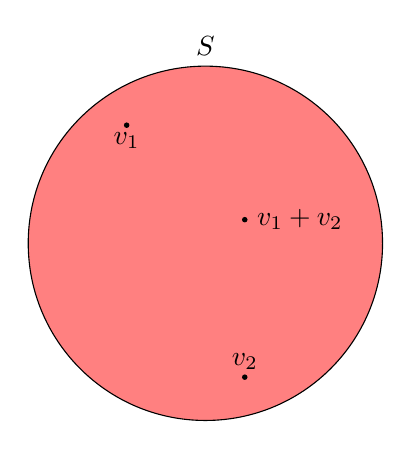
\begin{tikzpicture}
	
	% Circle with label
	\node[draw,
	circle,
	minimum size =4.5cm,
	fill=red!50,
	label=$S$] (circle1) at (0,0){};
	
	\node at (-1,1.3) {$v_1$};
	\node at (0.5,-1.5) {$v_2$};
	\node at (1.2,.3) {$v_1 + v_2$};
	
	%node[circle,fill,inner sep=1pt,label=above:](){};
	
	%\fill (a) circle[radius=1pt];
	\fill (-1, 1.5) circle[radius=1pt];
	\fill (0.5, -1.7) circle[radius=1pt];
	\fill (0.5, .3) circle[radius=1pt];
	
\end{tikzpicture}
\end{minipage}
\begin{minipage}{.45\linewidth}
$v = (x_1, \dots, x_n) \in \mathbb{R}^n$ \\
$0v = (0 \cdot x_1, \dots, 0 \cdot x_n) = (0, \dots , 0)$ \\
\textbf{\small CONDIZIONE NECESSARIA:} \\
$\color{red}\boxed{\normalcolor\textsf{Quindi ogni sottospazio di } \mathbb{R}^n \textsf{ contiene } 0\mathbb{R}^n}$
\end{minipage}

\flushleft\textbf{Domande:} \\
\begin{enumerate}
	\item \textsf{\small Un sottospazio è per definizione non vuoto; Può contenere un solo elemento?}
	\item \textsf{\small In generale quanti elementi contiene?}
\end{enumerate}

\textsf{\small \underline{Controesempio: }} \\
\(
T = \{ (1,1,1) , (2,1,4)\} \subseteq \mathbb{R}^3
\)\\
\textsf{\small \underline{NON} può essere un sottospazio di $\mathbb{R}^3$ perchè non contiene (0,0,0)} \\
\(
V = \{ (x,y) \in \mathbb{R}^2 \mid x + y = 1\}
\)\\
\textsf{\small \underline{NON} può essere un sottospazio di $\mathbb{R}^2$ perchè \underline{non} contiene $0\mathbb{R}^2 = (0,0)$ } \\
\vspace{0.2cm}
\textbf{Domanda:}
$S = {0\mathbb{R}^n}$ \textsf{\small è un sottospazio vettoriale di $\mathbb{R}^n$?}\\
\begin{itemize}
	\item \textsf{\small E' chiuso rispetto alla somma?} $0\mathbb{R}^n + 0\mathbb{R}^n = 0\mathbb{R}^n$
	\item \textsf{\small E' chiuso rispetto al prodotto per scalari?} $\forall \alpha \in \mathbb{R} \hspace{0.3cm} \alpha \cdot 0\mathbb{R}^n = 0\mathbb{R}^n \in S$
\end{itemize}

\textsf{\small \textcolor{red}{E' un sottospazio vettoriale di $\mathbb{R}^n$}} \\
$\{ 0\mathbb{R}^n\}$ \textsf{\small contiene $\boxed{\text{un solo}}$ elemento e si chiama \textcolor{red}{SOTTOSPAZIO BANALE}.} \\

$\boxed{\mathbb{R}^2 \subsetneq \mathbb{R}^3}$ \textsf{\small (non posso confrontare coppie con terne). NON solo NON è uno spazio vettoriale, ma non è neanche un sottoinsieme.}

\newpage

\(
\{ (x,y) \in \mathbb{R}^2 \mid \underbrace{x^2 + y = 0} _{y = -x^2} \}
\)
\textsf{\small è un sottospazio di $\mathbb{R}^2$?}\\
\textsf{\small ha infiniti elementi del tipo $(x, -x^2), x \in \mathbb{R}$}\\
\textsf{\small \textcolor{red}{MA non è un sottospazio perchè non è chiuso, ad esempio, rispetto al prodotto per scalari. Infatti:}}\\
\(
(1, -1) \in P \hspace{0.3cm}\text{\underline{MA}} -(1, -1) = \underbrace{(-1, 1)} _{y = -x^2 \text{ se } x = -1 \Rightarrow y = -(-1)^2 \Rightarrow y = -1} \notin P
\)

\textbf{Esempio:} \\
\(
S = \{ (x,\color{red}\boxed{\normalcolor y}\normalcolor) \in \mathbb{R}^2 \mid \color{red}\boxed{\normalcolor x = y}\normalcolor\}
\)\\
\(
= \{ (x, x) \mid x \in \mathbb{R}\}
\)\\
\noindent\begin{minipage}{.5\linewidth}
\begin{tikzpicture}
	\draw[<-]  (3.2,0) -- (-3.2, 0); % asse x
	\draw[<-] (0,3) -- (0,-3); % asse y
	
	\draw[->] (0,0) -- (3,2);
	\draw[->] (0,0) -- (1.5,1);
	\draw[->] (0,0) -- (-3,-2);
	
	%\node (x1) at (1.5, 1.2) {$ \vec{v} $};
	%\node (x2) at (-1.5, -1.2) {$ -\vec{v} $};
	
\end{tikzpicture}
\end{minipage}
\begin{minipage}{.45\linewidth}
\textsf{\small \underline{CHIUSO} RISPETTO ALLA SOMMA}\\
\textsf{\small \underline{CHIUSO} RISPETTO AL PRODOTTO PER SCALARI}\\
$\Rightarrow $ \textsf{\small è un sottospazio di $\mathbb{R}^2$} \\
\end{minipage}

\textbf{\underline{Esercizio}: } \textsf{\small Stabilire se $S = \{ (x,y) \in \mathbb{R}^2 \mid xy = 0\}$ è un sottospazio vettoriale di $\mathbb{R}^2$} \\

\textsf{\small Notiamo che $(1,0) \in S$ perchè soddisfa $\underbrace{1} _{x} \cdot \underbrace{0} _{y} = 0$ , analogamente $(0,1) \in S$ perchè soddisfa $0 \cdot 1 = 0$}\\
\textsf{\small MA $(1,0) + (0,1) = (1,1) \notin S$ perchè $1 \cdot 1 \neq 0$}\\
$\Rightarrow$ \textsf{\small S \underline{\underline{non}} chiuso rispetto alla somma , \underline{\underline{non}} è un sottospazio di $\mathbb{R}^2$}\\

\noindent\begin{minipage}{.5\linewidth}
	\begin{tikzpicture}
		\draw[<-]  (3.2,0) -- (-3.2, 0); % asse x
		\draw[<-] (0,3) -- (0,-3); % asse y
		
		\node (x) at (3.2, -0.2) { $x$ }; % la x
		\node (y) at (-0.2, 3) { $y$ }; % la y
		
		\draw[ForestGreen, ->] (0,0) -- (0,1);
		\draw[ForestGreen, ->] (0,0) -- (1,1);
		\draw[ForestGreen, ->] (0,0) -- (1,0);
		
		\node (x1) at (0, 1.2) {$ (0,1) $};
		\node (x2) at (1, 1.2) {$ (1,1) $};
		\node (x3) at (1, -0.3) {$(1,0) $};
		
	\end{tikzpicture}
\end{minipage}
\begin{minipage}{.45\linewidth}
	$xy = 0$ \\
	$x = 0$ oppure $ y = 0$ \\
	$S = \{ \underbrace{(x,y) \mid x = 0} _{\textcolor{red}{sottospazio}}\} \cup \{ \underbrace{(x,y) \mid y = 0} _{\textcolor{red}{sottospazio}}\}$
	\boxed{\textsf{\small (1,1) non appartiene non si trova sull'origine sull'asse x e y}}\\
	\textsf{\small \textcolor{red}{\underline{MA} la loro unione NON è un sottospazio perchè \underline{non} è chiusa rispetto alla somma}}\\
\end{minipage}
\textsf{\small Se prendiamo (solo una delle due rette): }\\
$ S_1 = \{(x,y) \in \mathbb{R}^2 \mid x = 0\} = \{(0,y) \in \mathbb{R}^2\}$\\
\textsf{\small è facile verificare che questo è un sottospazio di $\mathbb{R}^2$. Infatti se prendiamo:}\\
$ (0, a), (0,b) \in S_1 \hspace{0.3cm} (0, a) + (0, b) = (0, a + b) \in S_1$ \\
$\Rightarrow S_1$ chiuso rispetto alla somma. \\
analogamente\\
$\alpha \in \mathbb{R}, (0,a) \in S_1 , \alpha(0, a) = (0, \alpha a) \in S_1$
$\Rightarrow S_1$ chiuso rispetto al prodotto per scalari. \vspace{0.2cm} 

\textsf{\underline{Proposizione}:}\\
\textsf{\small Siano S,T due sottospazi vettoriali di $\mathbb{R}$, Allora $S \cup T$ è un sottospazio $\underset{\text{se e solo se}}{\Leftrightarrow}$ $S \subseteq T $ oppure $T \subseteq S$ (contenuto)}\\ \vspace{.2cm}
\textsf{\underline{Dim}.}\\
\textsf{\small Se $S \subseteq T$, $S \cup T = T$}\\
\noindent\begin{minipage}{.5\linewidth}
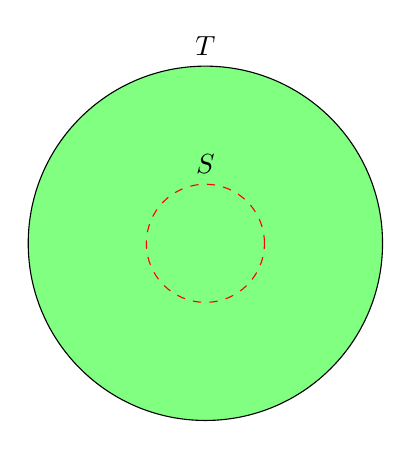
\begin{tikzpicture}
	
	% Circle with label
	\node[draw,
	circle,
	minimum size =4.5cm,
	fill=green!50,
	label=$T$] (circle1) at (0,0){};
	
	\node[draw,
	circle,dashed,red,
	minimum size =1.5cm,
	fill=green!50,
	label=$S$] (circle1) at (0,0){};
	
	
\end{tikzpicture}
\end{minipage}
\begin{minipage}{.45\linewidth}
\textsf{\small Analogamente se $T \subseteq S \hspace{.2cm} S \cup T = S $ che è un sottospazio per ipotesi supponiamo che $S \subsetneq T , T \subsetneq S $ e mostriamo che in tal viceversa caso $S \cup T$ \underline{non} può essere un sottospazio.}
\end{minipage}\\
\vspace{.5cm}
\noindent\begin{minipage}{.5\linewidth}
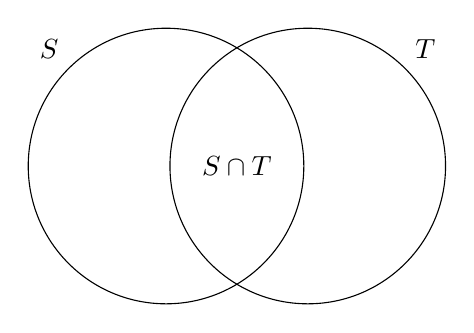
\begin{tikzpicture}
	
	% Set A
	\node [draw,
	circle,
	minimum size =3.5cm,
	label={135:$S$}] (S) at (0,0){};
	
	% Set B
	\node [draw,
	circle,
	minimum size =3.5cm,
	label={45:$T$}] (T) at (1.8,0){};
	
	% Set intersection label
	\node at (0.9,0) {$S\cap T$};
	
\end{tikzpicture}
\end{minipage}
\begin{minipage}{.45\linewidth}
\textsf{\small $S \underset{\text{intersecato}}{\cap} T$ è un sottospazio di $\mathbb{R}^n$?}\\
\textsf{\small Si lo è, perchè è chiuso rispetto alla somma e rispetto al prodotto per scalari.}
\end{minipage}\\ \vspace{.2cm}
\textsf{\small Gli esempi fatti mostrano che è possibile descrivere un sottospazio mediante equazioni lineari. \nolinebreak}\\
\textsf{\underline{Esempio 1}:}\\
\(
U = \{ (\textcolor{blue}{\boxed{\normalcolor x}},y,\color{green}\boxed{\normalcolor z}\normalcolor) \in \mathbb{R}^3 \mid \color{blue}\boxed{\normalcolor x = y}\normalcolor, \color{green}\boxed{\normalcolor z = 2y}\normalcolor \}
\)\\
\(
= \{ (\underbrace{y, y, 2y} _{y(1,1,2)}) \in \mathbb{R}^3\} \hspace{.1cm}\textsf{\small Ogni vettore di U è un multiplo di (1,1,2)}
\)\\
\enlargethispage{1\linewidth}
\textsf{\underline{Esempio 2}:}\label{esempio2} \\
\(
W = \{ (\textcolor{red}{\boxed{\normalcolor x}},y,\textcolor{orange}{\boxed{\normalcolor z}},t) \in \mathbb{R}^4 \mid \textcolor{red}{\boxed{\normalcolor x = -y}}, \textcolor{orange}{\boxed{\normalcolor z = 2t}}\}
\)\\
\(
= \{ (-y,y,2t,t) \mid y,t \in \mathbb{R}\} \hspace{.1cm} \textsf{\small (mi aspetto che $W \underset{\text{"assomiglia"}}{\simeq} \mathbb{R}^2$)}
\)\\
\(
y(-1,1,0,0) + t(0,0,2,1) 
\)\\
\textsf{\small \textcolor{red}{Ho descritto tutti gli $\infty$ elementi di W "\underline{in funzione}" di soli due.}}

% ======================= COMBINAZIONE LINEARE =================================

\newpage

\subsection{COMBINAZIONE LINEARE}

\begin{definition}[Combinazione Lineare]
	Siano $v_1, \dots , v_n \in \mathbb{R}^n$ Si chiama \textbf{COMBINAZIONE LINEARE} di $v_1, \dots , v_n$ ogni vettore $v \in \mathbb{R}^n$ della formula \\
	\centering $ v = \underbrace{\alpha_1} v_1 + \dots + \underbrace{\alpha_k} v_k \text{ con } \alpha_1, \dots , \alpha_k \in \mathbb{R}$ \\
	con $\alpha_1$ e $\alpha_k$ \textcolor{red}{coefficienti della combinazione lineare}
\end{definition}

\flushleft\textsf{\underline{Es}: Prendo due vettori}\\
\(
v_1 = (1,0,2) \hspace{.3cm} v_2 = (-1,3,2) \in \mathbb{R}^3
\)\\
\(
v = 3(1,0,2) -2(-1,3,2) \text{ è una combinazione lineare di $v_1,v_2$}
\)\\
\(
0\mathbb{R}^3 = 0v_1 + 0v_2 \hspace{.3cm} \text{ è sempre una combinazione lineare}
\)\\

\textsf{\small Nell'esempio 2, qui sopra a pag.\pageref{esempio2}, ho mostrato che $\boxed{\text{ogni}}$ vettore di W è combinazione lineare dei vettori (-1,1,0,0) e (0,0,2,1)}\\

% ====================== GENERATORI ==============================================

\subsection{Generatori}

\begin{definition}[Generatori]
	un sottospazio vettoriale S di $\mathbb{R}^n$ si dice \underline{generatore} dai vettori $v_1, \dots, v_k$ se \underline{ogni} vettore $v \in S$ si scrive come combinazione lineare di $v_1, \dots, v_k$
\end{definition}

\textsf{\underline{Esempio}:}\\
\textsf{\small W è generato da (-1,1,0,0) e (0,0,2,1) o, equivalentemente, dico che (-1,1,0,0) e (0,0,2,1) sono \textbf{GENERATORI} di W.}\\

\textsf{\underline{Nota}: Quando parlo di sottospazi di $\mathbb{R}^n$ intendo anche $\mathbb{R}^n$. Se voglio escludere $\mathbb{R}^n$ e lo spazio banale dico che il sottospazio è \textbf{\underline{PROPRIO}}.}\\
\vskip.2cm
\textsf{\underline{Domanda}: Con quali vettori è possibile generare $\mathbb{R}^2$?}\\

\textsf{\small Possiamo generare $\mathbb{R}^2$,con i vettori (1,0) e (0,1). Infatti $\forall v \in \mathbb{R}^2$ v = (a,b) = a(1,0) + b(0,1) con a,b $\in \mathbb{R}$}\\
$\Rightarrow \{ (1,0) (0,1)\}$ generano $\mathbb{R}^2$ \\

\noindent\begin{minipage}{.5\linewidth}
\begin{tikzpicture}
	\draw[<-]  (3,0) -- (-3, 0); % asse x
	\draw[<-] (0,3) -- (0,-3); % asse y
	
	%\node[below] (x) at (3.0, -0.3) { $x$ }; % la x
	%\node[left] (y) at (-0.3, 3) { $y$ }; % la y
	
	\node[left] at (0, 3) { $y$ };
	\node[below] at (3, 0) { $ x $ };
	
	\draw[ForestGreen, ->] (0,0) -- (0,1);
	\draw[ForestGreen, ->] (0,0) -- (1,1);
	\draw[ForestGreen, ->] (0,0) -- (1,0);
	
	\node (x1) at (0, 1.2) {$ (0,1) $};
	\node (x2) at (1, 1.2) {$ (1,1) $};
	\node (x3) at (1, -0.3) {$(1,0) $};
	
	\draw[ForestGreen, ->] (0,0) -- (0,-1);
	\draw[ForestGreen, ->] (0,0) -- (-1,-1);
	\draw[ForestGreen, ->] (0,0) -- (-1,0);
	
	\draw[ForestGreen, ->] (0,0) -- (-1,1);
	\draw[ForestGreen, ->] (0,0) -- (1,-1);
\end{tikzpicture}
\end{minipage}
\begin{minipage}{.45\linewidth}
\textsf{\small Riesco a riempire tutto il piano, riesco a riempire di vettori tutto il piano. E' per questo che (0,1) e (1,0) funzionano.}
\end{minipage}

\newpage

\textsf{\textcolor{red}{\underline{Domanda}:} E' possibile generare $\mathbb{R}^2$ con 3 vettori?}\\

\textsf{\small Se i primi due generano $\mathbb{R}^2$, allora il terzo va bene.}\\\vskip.5cm

\textsf{\textcolor{red}{\underline{Domanda}:} E' possibile generare $\mathbb{R}^2$ con un solo vettore?}\\

\textsf{\small \underline{\underline{NO}},perchè dato $v \neq 0$ i vettori della forma $\alpha v$ con $\alpha \in \mathbb{R}$ sono vettori che giacciono sulla stessa retta di V.}\\ 

\begin{tikzpicture}
	\draw[->] (0,0) -- (2,1);
	\draw[->] (0,0) -- (1,0.5);
	\draw[->] (0,0) -- (-2,-1);
	\draw[->] (0,0) -- (-1,-0.5);
	
	\node (v) at (0, 0.2) {$ v $};
\end{tikzpicture}

\textsf{\underline{Oss}. Per generare $\mathbb{R}^2$ servono almeno 2 vettori.}\\\vskip.5cm

\textsf{\textcolor{red}{\underline{Domanda}:} Bastano due vettori qualsiasi?}\\

\textsf{\small $\boxed{\text{NO}}$, Non devono essere allineati cioè non devono essere uno multiplo dell'altro. (perchè resterei sempre sulla stessa retta)}\\ \vskip.5cm

\textsf{\textcolor{red}{\underline{Domanda}:} Cosa succede nel caso di $\mathbb{R}^3$?}\\
\textsf{\small Un vettore solo non basta.}\\
\textsf{\textcolor{red}{\underline{Domanda}:} Due vettori non allineati bastano a generare $\mathbb{R}^3$?}\\
\textsf{\small Riesco mediante combinazioni lineari a generare tutti i vettori del piano individuato dai due vettori, ma non riesco a trovare nessun vettore che esce dal terzo piano.}\\
\textsf{\small 2 vettori $\boxed{\text{NON}}$ bastano a generare $\mathbb{R}^3$. Non riescono ad avere tutte le possibili somme. Ne servono almeno 3.}\\
\textsf{\small Per esempio: $\{ (1,0,0), (0,1,0), (0,0,1)\}$}\\ \vskip.5cm

\subsection{SOTTOSPAZIO GENERATO}

\begin{definition}[Sottospazio generato]
	Siano $v_1, \dots, v_k$ vettori di $\mathbb{R}^n$. Si chiama \textcolor{red}{SOTTOSPAZIO GENERATO} da $v_1, \dots, v_k$ e si indica con $<v_1, \dots, v_k>$ l'insieme di tutte e sole le combinazioni lineari di $v_1, \dots, v_k$ cioè: \\
	\centering $<v_1, \dots, v_k> = \{ \underbrace{\sum_{i=1}^{k} \alpha_i v_i \mid \alpha_i \in \mathbb{R}\}} _{\alpha_i v_1 + \dots + \alpha_k v_k}$
\end{definition}

\flushleft\textsf{\underline{Oss}. $<v_1, \dots, v_k>$ è un sottospazio vettoriale di $\mathbb{R}^n$}\\
\textsf{\small Osserviamo prima di tutto che $0\mathbb{R}^n = 0v_1 + \dots + v_k \in S$.}\\

% ---------------- SOMMA DI SOTTOSPAZI VETTORIALI ----------------------------

\subsection{SOMMA DI SOTTOSPAZI VETTORIALI}
\enlargethispage{1\linewidth}
\begin{definition}[Somma di Sottospazi Vettoriali]
	Siano S,T sottospazi vettoriali di $\mathbb{R}^n$. Si chiama \textbf{SOMMA} di S e T il sottoinsieme: \\
	\centering \( S + T \{ v = s + t \mid s \in S, t \in T\}\)
\end{definition}

\newpage
\textsf{\underline{Oss.1}: $S, T \subset S + T$ infatti ogni elemento di S si può pensare come $t = 0\mathbb{R}^n + t \in S + T$}\\
\textsf{\small Questo è equivalente a dire che $\boxed{\underbrace{S \cup T \subset S + T} _{\text{è costituito dagli elementi di S e dagli elementi di T.}}}$}\\

\textsf{\underline{Oss.2}: In particolare $0\mathbb{R}^n \in S \cap T$ certamente appartiene a $S + T =$ (Anche perchè $0\mathbb{R}^n = 0\mathbb{R}^n + 0\mathbb{R}^n$)}\\

\noindent\begin{minipage}{.5\linewidth}
	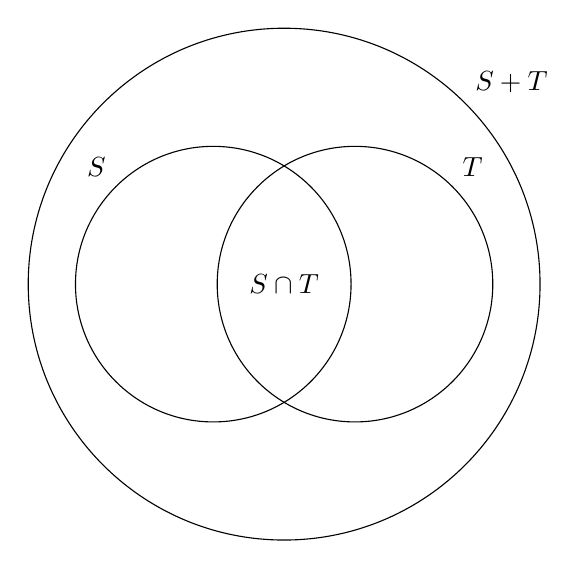
\begin{tikzpicture}
		
		% Set A
		\node [draw,
		circle,
		minimum size =3.5cm,
		label={135:$S$}] (S) at (0,0){};
		
		% Set B
		\node [draw,
		circle,
		minimum size =3.5cm,
		label={45:$T$}] (T) at (1.8,0){};
		
		% Set intersection label
		\node at (0.9,0) {$S\cap T$};
		
		%\draw (5,0) ellipse [radius=1.5cm];
		
		\node [draw,
		circle,
		minimum size =6.5cm,
		label={45:$S + T$}] (S+T) at (0.9,0){};
		
	\end{tikzpicture}
\end{minipage}
\begin{minipage}{.45\linewidth}
$ \hspace{1cm}\boxed{S \cap T \subseteq S \cup T \subseteq S + T}$
\end{minipage}

\textsf{\underline{Domanda}: L'unione di due sottospazi coincide con la loro somma?}\textsf{\small \textcolor{red}{\underline{\underline{NO!}}}}\\

\textsf{\underline{Prop}.: La somma di due sottospazi è un sottospazio.}\\
\(
\boxed{\underbrace{S \cup T \subsetneq S + T} _{\text{non sono la stessa cosa}}}
\)
\(
\boxed{S + T \text{è $\mathbb{R}^2$}}
\)
\(
\boxed{S \cup T \text{è l'unione degli assi}}
\)\\
\textsf{\small Abbiamo visto prima che: $\boxed{S + T = <S \cup T>}$}\\
\vskip.25cm
\textsf{\underline{Esercizio}: Stabilire se i vettori (0,0,1),(2,1,0),(1,1,1) generano $\mathbb{R}^3$.}\\
\vskip.15cm
\textsf{\underline{Svolgimento 1}: Devo capire se ogni vettore di $\mathbb{R}^3$ si può scrivere come una combinazione lineare di (0,0,1),(2,1,0),(1,1,1) cioè se $\forall(a,b,c) \in \mathbb{R}^3$ esistono dei coefficienti $\alpha, \beta, \gamma \in \mathbb{R}$ tale che $(a,b,c) = \alpha(0,0,1) + \beta(2,1,0) + \gamma(1,1,1) \Leftrightarrow$}\\

$(a,b,c) = (2\beta + \gamma, \beta + \gamma, \alpha + \gamma)$\\
\textsf{\small Sistema lineare nelle incognite $\alpha, \beta, \gamma$}\\

\(
\begin{cases*}
	2\beta + \gamma = a \\
	\beta + \gamma = b \\
	\alpha + \gamma = c
\end{cases*}
\)
\(
\text{1ª equazione - 2ª equazione $\rightarrow$}
\)
\(
\begin{cases*}
	\beta = a - b \\
	\gamma = b - \beta = b - a + b = 2b - a \\
	\alpha = c - \gamma = c - 2b + a
\end{cases*}
\)\\

\(
\Rightarrow \forall(a,b,c) \in \mathbb{R}^3
\)\\
\(
(a,b,c) = (\underbrace{c - 2b + a} _{\alpha})(0,0,1) + (\underbrace{a-b} _{\beta})(2,1,0) + (\underbrace{2b-a} _{\gamma})(1,1,1)
\)\\
$\Rightarrow$ \textsf{\small I vettori (0,0,1),(2,1,0),(1,1,1) generano $\mathbb{R}^3$.}\\

% ===================== LINEARMENTE INDIPENDENTE ================================

\newpage

\subsection{Linearmente Indipendente}
\begin{definition}[Linearmente Indipendente]
	k vettori $v_1, \dots, v_k$ di $\mathbb{R}^n$ si dicono linearmente \textcolor{red}{INDIPENDENTI} se l'unico modo di scrivere il vettore nullo come loro combinazione lineare è a coefficienti nulli. In caso contrario i vettori si dicono linearmente DIPENDENTI.
\end{definition}

\textsf{\underline{Riflettiamo}: E' sempre vero che}\\
$ 0v_1 + 0v_2 + \dots + 0v_k = 0\mathbb{R}^n$\\
\textsf{\small Non è detto che questo sia l'unico modo di scrivere $0\mathbb{R}^n$ come combinazione lineare di $v_1, \dots, v_k$.}\\
\textsf{\underline{Es}.} $v_1 = (1,0,0) \hspace{0.3cm} v_2 = (0,1,0) \hspace{0.3cm} v_3 = (2,1,0)$\\
$2(1,0,0) + (0,1,0) - (2,1,0) = (0,0,0)$\\
$\Rightarrow \{ v_1, v_2, v_3\}$ sono LINEARMENTE DIPENDENTI.\\
\textsf{\underline{Invece}}\\
$(0,0,0) = \alpha(1,0,0) + \beta(0,1,0) = (\alpha, \beta, 0) \Leftrightarrow \alpha = 0 , \beta = 0$\\
$\Rightarrow \{ (1,0,0),(0,1,0)\}$ sono LINEARMENTE INDIPENDENTI.\\
\centering \textsf{\underline{Guardiamo la definizione più da vicino}}\\
\flushleft $\boxed{k = 1}$ Un vettore $v_1$ è LINEARMENTE INDIPENDENTE se posso scrivere \centering$0\mathbb{R}^n = \underbrace{\alpha} _{0} v_1$\\
\flushleft$\Leftrightarrow \underbrace{\frac{1}{\alpha}} _{0\mathbb{R}^n} \cdot 0\mathbb{R}^n = \frac{1}{\color{red}\cancel{\normalcolor\alpha}}\color{red}\cancel{\normalcolor\alpha} \normalcolor v_1 = \color{red}\boxed{\normalcolor v_1}$\normalcolor\\
\textsf{\small cioè $\boxed{\text{un vettore}}$ v è linearmente indipendente $\underset{\text{se e solo se}}{\Leftrightarrow} v \neq 0\mathbb{R}^n$}\\
$\boxed{k = 2}$ 2 vettori $v_1, v_2$ sono linearmente DIPENDENTI se posso scrivere $0\mathbb{R}^n$ come loro combinazione lineare con coefficienti non tutti nulli, cioè \\
\(
0\mathbb{R}^n = \alpha_1 v_1 + \alpha_2 v_2 \hspace{.3cm} \frac{\alpha_1,\alpha_2 \in \mathbb{R}}{\text{con} (\alpha_1,\alpha_2) \neq (0,0)}
\)\\
\textsf{\small Per fissare le idee supponiamo che sia $\alpha_1 \neq 0$ allora}\\
$\Leftrightarrow v_1 = - \frac{\alpha_2}{\alpha_1}v_2$ uno è multiplo dell'altro (giacciono sulla stessa retta).\\
$\color{red}\boxed{\normalcolor \text{Equivalentemente, 2 vettori si dicono linearmente indipendenti se \underline{non} sono uno multiplo dell'altro.}}$\\

$\boxed{\text{k qualsiasi}} v_1, \dots, v_k $ sono linearmente DIPENDENTI se posso scrivere $0\mathbb{R}^n = \alpha_1 v_1 + \dots + \alpha_k v_k \hspace{0.3cm} \alpha_i \in \mathbb{R}$ con $ (\alpha_1,\dots,\alpha_k) \neq (0,\dots,0)$\\
\textsf{\small Per fissare le idee sia $\alpha \neq 0 \Leftrightarrow v_1 = \frac{-\alpha_2}{\alpha_1}v_2 - \dots - \frac{\alpha_k}{\alpha_1}v_k \Leftrightarrow$ uno di essi è combinazione lineare degli altri $\Leftrightarrow v_1 \in <v_2,\dots,v_k>$}\\
\textsf{\small \underline{Oss}. Mettendo insieme le definizioni di vettori linearmente indipendenti e di sottospazio generato da k vettori possiamo dire che}
\[
<v_1,\dots,v_k> = <v_1,\dots,v_{k-1}> \Leftrightarrow \{ v_1, \dots, v_k\}
\]
\textsf{\small sono linearmente dipendenti (se $v_k$ è combinazione lineare degli altri.) In altre parole un insieme di generatori si può rimpicciolire $\underset{\text{se e solo se}}{\Leftrightarrow}$ tali generatori sono linearmente dipendenti.}\\
\textsf{\small \underline{Esempio}: Consideriamo il sottospazio di $\mathbb{R}^3$}\\
\[
S = \{ (x,y,z) \in \mathbb{R}^3 \mid x - 2y + z = 0\}
\]
\textsf{\small Osserviamo che : } \centering$(1,0,0) \notin S$\\
$(0,1,0) \notin S$ \\
$(0,0,1) \notin S$ \\
\flushleft
\(
S = \{ \underbrace{(2y - z, y, z)} _{y(2,1,0) + z(-1,0,1)} \in \mathbb{R}^3\} = <(2,1,0),(-1,0,1)>
\)\\

\textsf{\small In particolare questo mostra che può capitare che $v_1,v_2 \notin S$ ma $2v_1 + v_2 \in S$}\\
\textsf{\small Quindi quello che può capitare, dato un sottospazio S è:}\\
\noindent\begin{minipage}{.5\linewidth}
	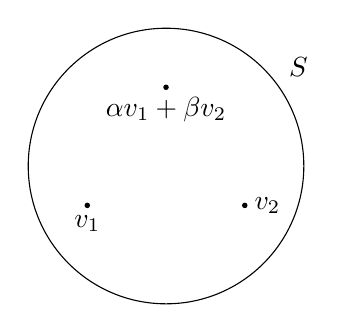
\begin{tikzpicture}
		
		% Set A
		\node [draw,
		circle,
		minimum size =3.5cm,
		label={35:$S$}] (S) at (0,0){};
		
		\fill (1, -0.5) circle[radius=1pt];
		
		\node[right] (v2) at (1, -0.5) {$v_2$};
		
		\fill (-1, -0.5) circle[radius=1pt];
		
		\node[below] (v1) at (-1, -0.5) {$v_1$};
		
		\fill (0, 1) circle[radius=1pt];
		
		\node[below] (v12) at (0, 1) {$\alpha v_1 + \beta v_2$};
		
	\end{tikzpicture}
\end{minipage}
\begin{minipage}{.45\linewidth}
\textsf{\large \underline{\underline{CHIUSO}}!}
\end{minipage}\vskip2.5mm
\noindent\begin{minipage}{.5\linewidth}
	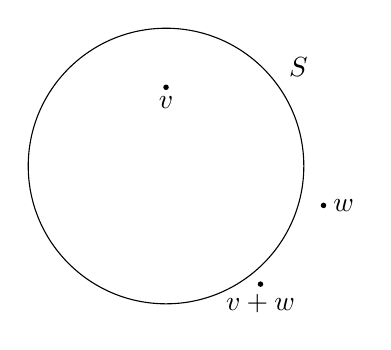
\begin{tikzpicture}
		
		% Set A
		\node [draw,
		circle,
		minimum size =3.5cm,
		label={35:$S$}] (S) at (0,0){};
		
		\fill (2, -0.5) circle[radius=1pt];
		
		\node[right] (w) at (2, -0.5) {$w$};
		
		\fill (1.2, -1.5) circle[radius=1pt];
		
		\node[below] (vw) at (1.2, -1.5) {$v + w$};
		
		\fill (0, 1) circle[radius=1pt];
		
		\node[below] (v) at (0, 1) {$v$};
		
	\end{tikzpicture}
\end{minipage}
\begin{minipage}{.45\linewidth}
$v \in S$\\
$w \notin S$\\
$v + w \notin S$
\end{minipage}\vskip2.5mm
\noindent\begin{minipage}{.5\linewidth}
	\begin{tikzpicture}
		
		% Set A
		\node [draw,
		circle,
		minimum size =3.5cm,
		label={35:$S$}] (S) at (0,0){};
		
		\fill (2, -0.5) circle[radius=1pt];
		
		\node[right] (w) at (2, -0.5) {$w$};
		
		\fill (1.2, -1.5) circle[radius=1pt];
		
		\node[below] (w2) at (1.2, -1.5) {$2_2$};
		
	\end{tikzpicture}
\end{minipage}
\begin{minipage}{.45\linewidth}
\textsf{\small Può capitare che $w_1 + w_2 \in S$ oppure $w_1 + w_2 \notin S$}
\end{minipage}
\textsf{\small \underline{Oss}. Se $V \subseteq \mathbb{R}^n$ è un sottoinsieme che non è un sottospazio \underline{\underline{NON}} posso parlare di generatori di V.}\\
\textsf{\small Certo posso considerare il sottospazio generato da V cioè $ <V>$.}\\

% =========================== BASE ==============================================

\newpage

\subsection{BASE}

\begin{definition}[Base]
	Dato un sottospazio vettoriale $S \subseteq \mathbb{R}^n$ si dice \underline{BASE} di S, un insieme di generatori di S linearmente indipendenti.\\
	Alla luce di quanto detto finora osserviamo che una base è un insieme minimale di generatori.
\end{definition}

\subsection{Dimensione}

\begin{theorem}
	Dato uno spazio vettoriale S di $\mathbb{R}^n$ ogni base di S ha la stessa cardinalità (cioè lo stesso numero di elementi). Chiamiamo \textcolor{red}{DIMENSIONE} di S, il numero di elementi di ogni sua base che indicheremo con \textcolor{red}{dim S}.
\end{theorem}

\textsf{\underline{Esempi}: Una base di $\mathbb{R}^2$ è $\{ (1,0),(0,1)\}$ infatti:}\\
\begin{itemize}
	\item \textsf{\small $\forall (a,b) \in \mathbb{R}^2, (a,b) = a(1,0) + b(0,1)$}
	\item \textsf{\small $\{ (1,0),(0,1)\}$ sono linearmente indipendenti perchè $\boxed{\text{non}}$ sono uno multiplo dell'altro.}
\end{itemize}

$\Rightarrow = \{ (1,0),(0,1)\}$ è una base di $\mathbb{R}^2 \Rightarrow \text{dim } \mathbb{R}^2 = 2$\\

\textsf{\small A questa base di $\mathbb{R}^2$ diamo un nome.}\\
\textsf{\small La chiamiamo \textcolor{red}{BASE CANONICA} di $\mathbb{R}^2$}\\
\textsf{\small \underline{\underline{Attenzione}}! Una base si intende \underline{\underline{ordinata}}.}\\
\textsf{\small Quindi $\{ (0,1),(1,0)\}$ è un'altra base di $\mathbb{R}^2$ (diversa dalla base canonica).}\\

\textsf{\underline{Esercizio}: Consideriamo i seguenti vettori $\mathbb{R}^4$:}\\
\begin{align*}
	v_1 &= (1,1,0,1) , v_2 = (1,1,0,0) , v_3 = (0,0,0,0)\\
	v_4 &= (2,2,0,3) , v_5 = (1,0,1,1) , v_6 = (2,0,2,0)\\
	v_7 &= (1,7,3,2)\\
\end{align*}
\enlargethispage{1\linewidth}
\textsf{\small \underline{Problema}: generano $\mathbb{R}^4$? Estrarre una base.}\\
\textsf{\small \underline{Svolgimento}: Sappiamo che i vettori (1,0,0,0),(0,1,0,0),(0,0,1,0),(0,0,0,1) generano $\mathbb{R}^4$.}\\
\textsf{\small Basta vedere se questi 4 vettori sono generati da $v_1, v_2,\dots, v_7$}\\
\textsf{\small Osserviamo che:}
\begin{align*}
	v_1 - v_2 &= (0,0,0,1)\\
	v_2 &= (1,1,0,0)\\
	v_6 &= (2,0,2,0) \Leftarrow (1,0,1,0)\\
	v_7 - 2(0,0,0,1) &= (1,7,3,0)\\
	(1,7,3,0) - (1,1,0,0) &= (0,6,3,0)\\
\end{align*}

\newpage

\begin{align*}
	(1,0,0,0) &\overset{?}{=} a(1,1,0,0) + b(1,0,1,0) + c(0,6,3,0)\\
	&= (a + b, a + 6c, b + 3c, 0)\\
\end{align*}

\(
\Leftrightarrow
\begin{cases*}
	a + b = 1 \\
	a + 6c = 0\\
	b + 3c = 0
\end{cases*}
\)
\(
\Leftrightarrow
\begin{cases*}
	a = -6c\\
	b = -3c\\
	-9c = 1
\end{cases*}
\)
\(
\Leftrightarrow
\begin{cases*}
	a = \frac{2}{3}\\
	b = \frac{1}{3}\\
	c = -\frac{1}{9}
\end{cases*}
\)

\begin{align*}
	v_2 - (1,0,0,0) &= (0,1,0,0)\\
	(1,0,1,0) - (1,0,0,0) &= (0,0,1,0)
\end{align*}

\begin{itemize}
	\item \textsf{\small Cosa significa "estrarre" una base di un insieme di generatori?}
\end{itemize}\vskip-1mm
\textsf{\small Base = insieme di generatori linearmente indipendenti.}\\
\textsf{\small Supponiamo che $\{ v_1, \dots, v_k\}$ siano generatori di un sottospazio s di $\mathbb{R}^n$ cioè $S = <v_1, \dots, v_k>$. $\{ v_1, \dots, v_k\}$ è una base di S? cioè $\{ v_1, \dots, v_k\}$ sono linearmente indipendenti?}\\

\noindent\begin{minipage}{.5\linewidth}
	$\boxed{\text{NO}}$\\
	\textsf{\small Uno di essi, diciamo $v_k$, è combinazione lineare degli altri.}\\
	\textsf{\small In tal caso:}
\end{minipage}
\begin{minipage}{.45\linewidth}
	$\boxed{\text{SI}}$\\
	\textsf{\small Ho trovato una base.}\\
\end{minipage}
\centering $S = <v_1, \dots, v_{k-1}, v_k> = \underbrace{<v_1, \dots, v_{k-1}>} _{\text{generano S , sono linearmente indipendente?}}$?

\flushleft
\begin{minipage}{.5\linewidth}
	$\boxed{\text{NO}}$\\
	$\{ v_1, \dots, v_{k-1} \} \text{sono lin. ind.} $\\
	$ \Leftrightarrow \text{Uno di essi è comb. lin. degli altri}$\\ $\Rightarrow \text{lo scarto}$.\\
\end{minipage}
\begin{minipage}{.45\linewidth}
	$\boxed{\text{SI}}$\\
	$\Rightarrow \{ v_1, \dots, v_{k-1}\} \text{è una base di S}$.
\end{minipage}
\vskip 2mm
\textsf{\small Itero il procedimento finchè non trovo un insieme \underline{\underline{minimale}} di generatori cioè un insieme di generatori di S lin. indipendenti (una \underline{\underline{base}})}\\
\textsf{\small Torniamo all'esercizio :}\\

\textsf{\small Trovare base, ovvero dai 7 vettori dati, trpvarne 4 che generano $\mathbb{R}^4$ e sono linearmente indipendenti e quindi una base.}\\

\(
\mathbb{R}^4 = <\color{red}\boxed{\normalcolor v_1}\normalcolor, \color{red}\boxed{\normalcolor v_2}\normalcolor, v_3, v_4, \color{red}\boxed{\normalcolor v_5}\normalcolor, v_6, \color{red}\boxed{ \normalcolor v_7 }\normalcolor>
\)
\begin{align*}
	\boxed{v_1} &= (1,1,0,1) , \boxed{v_2} = (1,1,0,0), v_3 = (0,0,0,0)\\
	v_4 &= (2,2,0,3), \boxed{v_5} = (1,0,1,1), v_6 = (2,0,2,0)\\
	\boxed{v_7} &= (1,7,3,2)\\
\end{align*}

\(
v_4 \overset{?}{\in} <v_1, v_2> \Leftrightarrow (2,2,0,3) = a(1,1,0,1) + b(1,1,0,0) = (a + b, a + b, 0, a)
\)
\centering
\(
a = 3 , b = -1
\)
%\flushleft
$\Rightarrow \in <v_1, v_2>$\\
\(
v_5 \overset{?}{\in} <v_1, v_2> \Leftrightarrow (1,0,1,1) = \alpha(1,1,0,1) + \beta(1,1,0,0) 
\)
\(
= (\alpha + \beta, \alpha + \beta, 0, \alpha)
\)
\(
\Leftrightarrow
\begin{cases*}
	\alpha + \beta = 1 \\
	\alpha + \beta = 0 \\
\end{cases*}
\)\\
\(
v_5 \notin <v_1, v_2> \Leftrightarrow v_5 \text{ è lin. indip. da } v_1, v_2
\)\\
\(
v_6 \overset{?}{\in} <v_1, v_2, v_5>
\)
\(
(2,0,2,0) \overset{?}{=} a(1,1,0,1) + b(1,1,0,0) + c(1,0,1,1) = (a + b + c, a + b, c, a + c) 
\)
\(
\Leftrightarrow
\begin{cases}
	a + b + c = 2 \\
	a + b = 0 \\
	c = 2 \\
	a + c = 0 \\
\end{cases}
\)
\(
\Leftarrow
\begin{cases*}
	b = 2 \\
	c = 2 \\
	a = -2 \\
\end{cases*}
\)
\(
\Rightarrow
(2,0,2,0) \in <v_1, v_2, v_5>
\)\\
\(
v_7 \overset{?}{\in} <v_1, v_2, v_5>
\)
\(
(1,7,3,2) \overset{?}{=} a(1,1,0,1) + b(1,1,0,0) + c(1,0,1,1) = (a + b + c, a + b, c, a + c)
\)
\(
c \Rightarrow
\begin{cases*}
	a + b + c = 1 \\
	a + b = 7 \\
	c = 3 \\
	a + c = 2 \\
\end{cases*}
\)
\(
a + b + c = 10
\)\\
\(
(1,7,3,2) \notin <v_1, v_2, v_5> \Leftrightarrow \{ v_1, v_2, v_5, v_7\} \text{sono linearmente indipendenti} \Rightarrow <v_1, \dots, v_7> = <v_1, v_2, v_5, v_7> = \mathbb{R}^4
\)\\

\flushleft\textsf{\small \underline{Esempio}: Sia $S = \{ (x,y,z,t) \in \mathbb{R}^4 \mid x - y + z - t = 0\}$}\\

\textsf{\small Osserviamo che (1,1,0,0) $ \in S$. Completare $\{ (1,1,0,0)\}$ in una base di S. (capiamo che (1,1,0,0) appartiene ad S perchè se lo sostituiamo nell'equazione viene = 0).}\\
\textsf{\small Osservo subito che $S \neq \mathbb{R}^4$ perchè, ad esempio, (1,0,0,0) $ \notin S $ (lo capiamo perchè sostituendolo nell'equazione non viene = a 0).}\\
\(
S \color{red}\boxed{\normalcolor \subsetneq \mathbb{R}^4} \normalcolor \text{sto dando per buono che S è un sottospazio (sarebbe da verificare).} 
\)\\
\(
\color{red} dim S \leq 3 \normalcolor
\)\\
\(
(0,1,1,0) \in S \text{ ed è lin. indip. da } (1,1,0,0) \text{ perchè \underline{\underline{non}} è un suo multiplo.}
\)\\
\(
(0,0,1,1) \in S. \text{ è lin. indip. da (1,1,0,0) e (0,1,1,0)?}
\)\\
\(
\color{red} \alpha(1,1,0,0) + \beta(0,1,1,0) = (\dots, 0) \normalcolor \boxed{\text{ SI }}  \text{ sono vettori lin. indipendenti in S}
\)
\(
\Rightarrow \{ (1,1,0,0), (0,1,1,0), (0,0,1,1)\} \text{ base di S.}
\)\\
\(
dim S \leq 3 \Rightarrow
\)
\textsf{\small Avrei potuto procedere cercando prima un insieme di generatori di S e poi "estraendo" da esso una base.}\\

\[
S = \{ (x,y,z,t) \mid x - y + z - t = 0\}
\]
\(
S = \{ \color{red}\boxed{\normalcolor(x,y,z,x - y + z)} \normalcolor \mid \color{red}\boxed{\normalcolor x - y + z - t = 0}\normalcolor \}
\)\\
\(
S = \{ (x,y,z,x - y + z) \in \mathbb{R}^4\} = \underbrace{<(1,0,0,1),(0,1,0,-1),(0,0,1,1)>} _{\text{sono lin. ind. ?}}
\)\\
\(
x(1,0,0,1) + y(0,1,0,-1) + z(0,0,1,1)
\)\\
\(
(1,0,0,1) \text{ è lin. indip. perchè non nullo}
\)\\
\(
(1,0,0,1) e (0,1,0,-1) \text{ sono lin. indip. perchè non sono uno multiplo dell'altro }
\)\\
\(
(0,0,1,1) \overset{?}{\in} <(1,0,0,1),(0,1,0,-1)> \boxed{\text{ NO }}
\)\\
\(
\Rightarrow \{ (1,0,0,1),(0,1,0,-1),(0,0,1,1)\} \text{ sono lin. indip.}
\)\\
\(
\Rightarrow \text{ individuo una base di S}
\)\\
$\Rightarrow dim S = 3$\\
\vskip.25cm
\textsf{\small Abbiamo visto che ci sono (almeno) 2 modi di costruire una base di un sottospazio $S \subseteq \mathbb{R}^4$}\\
\begin{enumerate}
	\color{red}\item \textcolor{red}{A partire da un insieme di vettori lin. indipendenti} \normalcolor
\end{enumerate}
\textsf{\small Aggiungo uno alla volta, vettori lin. indipendenti dai precedenti finchè non trovo un insieme di generatori.}\\
\centering\textsf{\underline{COMPLETAMENTO}}\\
\flushleft
\begin{enumerate}
	\color{red}\item[2.] A partire da un insieme di generatori \normalcolor
\end{enumerate}

\textsf{\small Elimino uno alla volta i generatori lin. indipendenti dagli altri finchè non trovo un insieme di vettori lin. indipendenti.}\\
\centering\textsf{\underline{ESTRAZIONE}}\\
\flushleft

$\boxed{\text{Problema}}$ \textsf{Come si fa a capire se 2 sottospazi di dimensione 2 $S = <v_1, v_2> , T = <w_1, w_2>$ coincidono?}\\

\textsf{\small \underline{Esempio}:} $\{ (0,a,b,0) \in \mathbb{R}^4 \} = S = <(0,1,0,0),(0,0,1,0)>$\\
\textsf{\small $\{ (0,0,a,b) \in \mathbb{R}^4\} = T = <(0,0,1,0),(0,0,0,1)>$}\\
$ S \neq T$ \textsf{\small perchè, per esempio, $\underbrace{(0,1,0,0)} _{S} \neq T$}\break

\textsf{\small Consideriamo ora una matrice 2x3 a coefficienti reali:}\\
\[
A =
\begin{pmatrix}
	&1 &-2 &3 \\
	&0 &1 &2 \\
\end{pmatrix}
\in M_{2,3}(\mathbb{R})
\]\\
\centering\textsf{\small Allora posso leggere le sue righe come vettori di $\mathbb{R}^3$}\\
\(
(1,-2,3),(0,1,2)
\)\\
\centering\textsf{\small Nello stesso modo posso leggere le sue colonne come vettori di $\mathbb{R}^2$}\\
\(
(1,0),(-2,1),(3,2)
\)\\
\textsf{\small Posso quindi considerare il sottospazio S di $\mathbb{R}^3$ generato dalle righe di A}\\
$S = <(1,-2,3),(0,1,2)>$ \textsf{\small e il sottospazio T di $\mathbb{R}^2$ generato dalle colonne di A}\\
$T = <(1,0),(-2,1),(3,2)>$\\
\textsf{\small Posso chiedermi quali siano le dimensioni di S e T dim S = 2, dim T = 2}\\
\textsf{\small Questo fatto succede sempre!! Vale a dire: data una matrice $A \in M_{m,n}(\mathbb{R})$ il sottospazio di $\mathbb{R}^n$ generato ($T = \mathbb{R}^2$) dai vettori riga di A e il sottospazio di $\mathbb{R}^n$ generato dai vettori colonna di A \underline{\underline{hanno}} sempre la stessa dimensione. Tale dimensione si chiama \underline{\underline{RANGO}} di A e si indica con $rg(A)$ (o $\underbrace{\text{rk}} _{\text{rank}}(A)$), Nell'esempio fatto rg A = 2.}\\
\textsf{\small \underline{rango matrici non a scala}}\\
\textsf{\small non numero di righe, ma linearmente indipendenti.}\\
\[
rg
\begin{pmatrix}
	&1 &1 &1 &1 \\
	&2 &2 &2 &2 \\
	&3 &3 &3 &3 \\
\end{pmatrix}
= 1
\]
\flushleft$\boxed{\text{Osserviamo}}$ \textsf{\small che rg A = 0 significa che il sottospazio generato delle righe di A è banale e così pure è banale il sottospazio generato dalle colonne quindi A = 0}\\

\textcolor{red}{ATTENZIONE!} \textsf{\small abbiamo definito \underline{il rango di una matrice a scala} come il numero delle sue righe non nulle (o, equivalentemente, il numero di pivot della matrice a scala).}\\
\textsf{\small \underline{\underline{Ora}} $\boxed{\text{dobbiamo}}$ scala le due definizioni di rango coincidono.}\\
\textsf{\small Righe non nulle sono linearmente indipendenti.}\\
\textsf{\small \underline{Esempio}}\\
\[
A =
\begin{pmatrix}
	&\color{red}\boxed{\normalcolor 1}\normalcolor &2 &3 &4 \\
	&0 &0 &\color{red}\boxed{\normalcolor 1}\normalcolor &2 \\
	&0 &0 &0 &\color{red}\boxed{\normalcolor 3}\normalcolor
\end{pmatrix}
\text{rg A} = 3
\]
\textsf{\small Le righe non nulle di una matrice a scala sono linearmente indipendenti quindi il sottospazio generato dalle righe di una matrice a scala ha dimensione data dal numero di righe non nulle.}\\

% ================= RANGO MATRICE A SCALA ========================================

\subsection{RANGO MATRICE A SCALA}

\begin{definition}[RANGO MATRICE A SCALA]
	Sia $A \in M_{m,n} \in (\mathbb{R})$. Si chiama rango di A e si indica con rg(A) il massimo numero di righe linearmente indipendenti di A (come vettori di $\mathbb{R}^n$) o, equivalentemente, il massimo numero di colonne linearmente indipendenti di A (come vettori di $\mathbb{R}^n$).\\
\end{definition}

\textsf{\small \underline{Ex}:}\\
\[
A =
%\left(
\begin{pmatrix}
	1 & -1  &  3\\
	0 & 1  &  2\\
	0 & 0  &  1\\
	3 & 1  &  3\\
\end{pmatrix}
%\right)
\in \text{M}_{4,3}(\mathbb{R}) \hspace{0.3cm} \text{rg A} = 3
\]\\
\enlargethispage{1\linewidth}
\textsf{\small \underline{Osservazione}: Supponiamo che $A \in M_{m,n} (\mathbb{R})$ sia una $\boxed{\text{matrice a scala}}$ allora abbiamo 2 definizioni di rango di A.}\\

\newpage
\centering\textsf{rg A}\\
\noindent\begin{minipage}{.35\linewidth}
\color{ForestGreen}\boxed{\textsf{\small \normalcolor il massimo numero di righe}} \\ \color{ForestGreen}\boxed{\textsf{\small \normalcolor o di colonne linearmente}}\\
\boxed{\textsf{\small \normalcolor indipendenti}}
\end{minipage}
\begin{minipage}{.25\linewidth}
\color{ForestGreen}\boxed{\textsf{\small \normalcolor numero di righe non nulle}}\\
\color{ForestGreen}\boxed{\textsf{\small \normalcolor = }}\\
\color{ForestGreen}\boxed{\textsf{\small \normalcolor il numero di pivot di A}}
\end{minipage}
\flushleft
\textsf{\small E' necessario osservare che, nel caso di matrici a scala, non c'è ambiguità, cioè che le due definizioni coincidono.}\\
\textsf{\small Basta mostrare che in una matrice a scala le righe non nulle sono linearmente indipendenti. Questo si può fare usando "l'argomento degli zeri" cominciando dalle righe in basso e risalendo.}\\
\textsf{\small \underline{Ex}.}\\
\[
A =
\begin{pmatrix}
	\color{ForestGreen}\boxed{\normalcolor -1} & 3 &  2 & 1\\
	0 & \color{ForestGreen}\boxed{\normalcolor 1}  &  2\\
	0 & 0  &  0 & \color{ForestGreen}\boxed{\normalcolor 1}\\
	0 & 0  &  0 & 0\\
\end{pmatrix}
\text{rg A} = 3 \text{ righe non nulle }
\]\\
\(
(0,0,0,1) \neq 0\mathbb{R}^4 \Rightarrow \text{ lin. ind.}
\)\\
\(
\{ (0,0,0,1),(0,1,2,2)\} \text{ lin. ind. perchè non sono uno multiplo dell'altro}
\)\\
\(
\{ (-1,3,2,1),(0,1,2,2),(0,0,0,1)\} \text{ sono lin. ind. perchè }
\)\\
\(
(-1,3,2,1) \notin <(0,1,2,2),(0,0,0,1)>
\)\\
\(
3 = \text{ dim } <(-1,3,2,1),(0,1,2,2),(0,0,0,1)>
\)\\
\textsf{\small Per quanto abbiamo detto, in questo esempio 3 è anche il numero di colonne linearmente indipendenti della matrice A. Notiamo infatti che le colonne contenenti i pivot sono lin. ind.}\\
$\{ (-1,0,0,0),(3,1,0,0),(1,2,1,0)\}$\\
\textsf{\small Abbiamo preso solo le colonne dove c'era il pivot.}\\
\textsf{\small La terza colonna, invece, è combinazione lineare delle prime 2:}\\
$(2,2,0,0) = 4(-1,0,0,0) + 2(3,1,0,0)$\\
\textsf{\underline{Problema}: Come si calcola (in modo efficiente) il rango di una matrice qualsiasi?}\\
\color{ForestGreen}\boxed{\textsf{FATTO}} \textsf{\small La risoluzione di Gauss preserva il rango.}\normalcolor \\
\textsf{\small Per calcolare il rango di una matrice qualsiasi A si può ridurre A a scala per righe ottenendo la matrice $A'$ e si ha \boxed{rg A = rg $A'$}}\\
$\boxed{\text{Attenzione}}$ \textsf{\small Questo significa che le operazioni elementari sulle righe di A preservano \underline{anche} la dimensione del sottospazio generato dalle colonne (perchè questa dimensione è sempre rg A)\underline{\underline{ MA }} le operazioni sulle righe non preservano il sottospazio generato dalle colonne.}\\
\enlargethispage{1\linewidth}
\textsf{\underline{Es}.}\\
\[
A =
\begin{pmatrix}
	1 & 2 \\
	3 & -1 \\
	1 & 1
\end{pmatrix}
\underset{\text{2ª riga = -3(1ª riga)}}{\overset{\text{3ª riga = 3ª riga - 1ª riga}}{\longrightarrow}}
\begin{pmatrix}
	1 & 2 \\
	0 & -7 \\
	0 & -1
\end{pmatrix}
\longrightarrow
\begin{pmatrix}
	1 & 2 \\
	0 & -1 \\
	0 & 0
\end{pmatrix}
= A'
\]\\

\newpage

\centering$<(1,2),(3,-1),(1,1)> = <(1,2),(0,-1),> = \mathbb{R}^2 \hspace{0.3cm} \text{rg A} = 2$\\

\textsf{\small rg A = rg $A'$, A ha 2 colonne lin. ind. così come A!}\\

$\boxed{\text{MA}} \hspace{0.3cm} <\underbrace{(1,3,1),(2,-1,1)}> \neq <\underbrace{(1,0,0),(2,-1,0)} _{z = 0}>$ \\

$\text{dim } 2 = <(1,3,1),(2,-1,1)> = \text{ dim } <(1,0,0),(2,-1,0)>$\\

\flushleft

\textsf{\underline{Esempio 3}: Siano $S = \{ (x,y,z) \in \mathbb{R}^3 \mid x - 2y + z = 0\}$ e $ T = \{ (x,y,z) \in \mathbb{R}^3 \mid y - z = 0\}$ Determinare una base di $S \cap T$ ed una base di $ S + T$.}\\

\textsf{\underline{Svolgimento}}\\

\textsf{\small Determiniamo } $S \cap T = \{ (x,y,z) \in \mathbb{R}^3 \mid x - 2y + z = 0, y - z = 0\}$\\

\[
\begin{cases*}
	x - 2y + z = 0 \\
	y - z = 0 \\
\end{cases*}
\Leftrightarrow
\begin{cases*}
	x = y \\
	y = z \\
\end{cases*}
= \{ (x,x,x) \in \mathbb{R}^3\}
\]\\
$=<(1,1,1)>$\\
$\{ (1,1,1)\}$ \textsf{\small è una base di $S \cap T \hspace{0.3cm} dim S \cap T = 1$}\\
\textsf{\small Ora determiniamo S + T}\\
\textsf{\underline{Osservazione}} \textsf{\small Siano S,T sottospazi vettoriali di $\mathbb{R}^n$.}\\
\textsf{\small sia $\{ v_1, \dots, v_k\}$ \color{ForestGreen}\underline{\normalcolor una base di S} \normalcolor e sia $\{ w_1, \dots, w_n\}$ una base di T. Quindi $ k = dim S, h = dim T$.}\\
\textcolor{red}{\underline{ATTENZIONE}! In generale $\{ v_1, \dots, v_k, w_1, \dots, w_h\}$ $\boxed{\text{non}}$ sono una base di S + T cioè in generale non è detto che $v_1, \dots, v_k, w_1, \dots, w_h$ siano lin. indipendenti}\\
\textsf{\small Infatti ogni vettore $v \in S + T$ si scrive $ v = s + t$ con}\\
\(
\underbrace{s \in S} _{s = \alpha_1 v_1 + \dots + \alpha_k v_k}, \underbrace{t \in T} _{t = \beta_1 w_1 + \dots + \beta_n w_n}
\)\\
$(\alpha_i \in \mathbb{R}) \hspace{0.6cm} (\beta_j \in \mathbb{R})$\\
$\Rightarrow v = s + t = \alpha_1 v_1 + \dots + \alpha_k v_k + \beta_1 w_1 + \dots + \beta_n w_n$\\

\textsf{\small Nel nostro esempio determiniamo S + T usando questa osservazione.}\\
\[
S = \{ (x,y,z) \in \mathbb{R}^3 \mid \underbrace{x - 2y + z = 0} _{z = 2y - x}\} = \{ (x,y,2y - x) \in \mathbb{R}^3\} =
\]\\
\centering$ = <(1,0,-1),(0,1,2)>$\\
\textsf{\small lin. indip.}\\
\flushleft
\textsf{\small \color{ForestGreen}\underline{\normalcolor Una base d S} \normalcolor è $\{ (1,0,-1),(0,1,2)\}$}\\
\(
T = \{ (x,y,z) \in \mathbb{R}^3 \mid \underbrace{y - z = 0} _{y = z}\} = \{ (x,y,y) \in \mathbb{R}^3 \} = <(1,0,0),(0,1,2)>
\)\\
\textsf{\small \color{ForestGreen}\underline{\normalcolor Una base di T }\normalcolor è $\{ (1,0,0),(0,1,1)\}$}\\
\textsf{\small Grazie all'osservazione che abbiamo fatto}\\
\(
S + T = <(1,0,-1),(0,1,2),(1,0,0),(0,0,1)>
\)\\
\[
\text{dim(S + T)} = \text{ rg }
\begin{pmatrix}
	1 & 0 & -1 \\
	0 & 1 & 2 \\
	1 & 0 & 0 \\
	0 & 1 & 1 \\
\end{pmatrix}
= \text{ rg }
\begin{pmatrix}
	1 & 0 & -1 \\
	0 & 1 & 2 \\
	0 & 0 & 1 \\
	0 & 1 & 1 \\
\end{pmatrix}
= \color{ForestGreen} \boxed{\normalcolor \underbrace{3}_{\text{rango}}} \hspace{0.3cm} \boxed{\normalcolor \text{S + T} \subseteq \mathbb{R}^3}
\]\\
\normalcolor $\Rightarrow\text{ S + T = $\mathbb{R}^3$}$\\ \vskip.5mm
$\boxed{\text{A questo punto scelgo la base di $\mathbb{R}^3$ che preferisco, per esempio, la base canonica.}}$\\ \vskip .25cm
\textsf{\underline{Osservazione}: {\small In questo esempio abbiamo:}}\\
\textsf{dim S = 2, dim T = 2, dim $S \cap T = 1$, dim S + T = 3}\\
\[
\color{ForestGreen}\boxed{\normalcolor \text{dim S + dim T - dim S $\cap$ T = dim (S + T)}}
\]
\centering\textcolor{ForestGreen}{Formula di Grassmann}\\

\subsection{Grassmann}

\flushleft \textsf{\underline{Vale la seguente formula}:}\\
\begin{theorem}[Grassmann]
	Siano S,T sottospazi vettoriali di $\mathbb{R}^n$\\
	Allora\\
	\[
	\text{ dim  (S + T) = dim S + dim T - dim (S$\cap$T)}
	\]
\end{theorem}

\textsf{$\boxed{\text{Idea}}$ :} \textsf{\small Calcolare la dimensione di un sottospazio di $\mathbb{R}^n$ significa contare gli elementi di una sua base.}\\
\textsf{\small In generale abbiamo visto che se $B_S \cup B_T$ individua un insieme di generatori di S + T $\boxed{\text{MA}}$ $B_S \cup B_T$ in generale \underline{NON} sarà una base di S + T.}\\

\textsf{\underline{Esempio}:}
\begin{align*}
	S = <(1,1,0),(0,1,1)> & B_S = \{ (1,1,0),(0,1,1)\} \\
	T = <(1,0,0),(0,0,1)> & B_T = \{ (1,0,0),(0,0,1)\}
\end{align*}
$S + T = \underbrace{<(1,1,0),(0,1,1),(1,0,0),(0,0,1)>} _{\text{\textcolor{ForestGreen}{\small \underline{non} sono lin. indipendenti perchè sono 4 vettori in $\mathbb{R}^3$!}}}$\\
\color{ForestGreen}$\Rightarrow$ \textsf{\small Non costituiscono una base di S + T}\\
\textsf{\small Per trovare una base di S + T devo scartare i vettori lin. dipendenti dagli altri.}\\
\textsf{\small Per esempio: (0,1,1) = (1,1,0) + (0,0,1) - (1,0,0) }\\
\normalcolor $\Rightarrow$ $ S + T = \underbrace{<(1,1,0),(1,0,0),(0,0,1)>} _{\textsf{\small sono lin. ind. $\Rightarrow$ una base}}$\\

 \textsf{\small S + T è $\{ (1,1,0),(1,0,0),(0,0,1)\}$, (dim S + T = 3 $\Rightarrow$ S + T = $\mathbb{R}^3$)}\\
 
 \newpage
 
 \textsf{\underline{Domanda}:} \textsf{\small C'è un modo per costruire direttamente una base di S + T (senza passare per un insieme di generatori più grande)?}\\ 

\color{black}
\normalcolor
\noindent\begin{minipage}{.5\linewidth}
	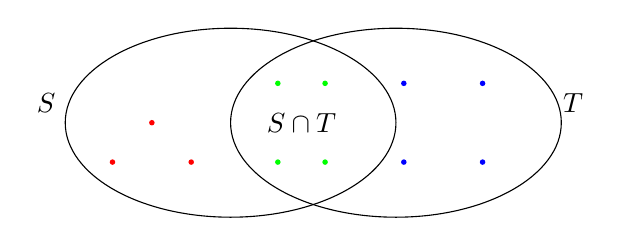
\begin{tikzpicture}
		
		\node[above left] at (-2.1,0) {$S$};
		
		\node[above right] at (4.1,0) {$T$};
		
		% in T
		\fill[blue] (3.2, -0.5) circle[radius=1pt];
		\fill[blue] (3.2, 0.5) circle[radius=1pt];
		\fill[blue] (2.2, -0.5) circle[radius=1pt];
		\fill[blue] (2.2, 0.5) circle[radius=1pt];
		
		% nell'intersezione
		\fill[green] (0.6, -0.5) circle[radius=1pt];
		\fill[green] (0.6, 0.5) circle[radius=1pt];
		\fill[green] (1.2, -0.5) circle[radius=1pt];
		\fill[green] (1.2, 0.5) circle[radius=1pt];
		
		% in S
		\fill[red] (-1, 0) circle[radius=1pt];
		\fill[red] (-0.5, -0.5) circle[radius=1pt];
		\fill[red] (-1.5, -0.5) circle[radius=1pt];
		
		\draw (0,0) ellipse (2.1cm and 1.2cm);
		
		\draw (2.1,0) ellipse (2.1cm and 1.2cm);
		
		% Set intersection label
		\node at (0.9,0) {$S\cap T$};
		
	\end{tikzpicture}
\end{minipage}
\begin{minipage}{.45\linewidth}
	$ \hspace{.3cm} \underbrace{7 + 8 - 4 = 11} _{\textsf{dim S + dim T - S$\cap$T}}$
\end{minipage}

\textsf{\underline{Domanda}}\\
\textsf{\small Possono esistere 2 sottospazi vettoriali di $\mathbb{R}^3$ di dimensione due la cui intersezione è banale?}\\
$\boxed{\text{NO}}$ \textsf{\small Perchè per la formula di Grassmann se S ha dimensione 2 e T ha dimensione 2, ma S,T $\subseteq \mathbb{R}^3$ anche S + T $\subseteq \mathbb{R}^3 \Rightarrow$ dim(S + T) = 2 + 2 - $\underbrace{dim S \cap T} _{\text{se fosse = 0}}$ = 4}\\
\textsf{\small Sarebbe impossibile (se l'intersezione fosse uguale a 0).}\\
\textsf{\small In questa situazione dim S$\cap$T $\geq$ 1}\\
\textsf{\small Geometricamente questo significa che in uno spazio tridimensionale due punti hanno in comune almeno una retta.}\\
\textsf{\small Riprendiamo l'esempio e costruiamo una base di S + T a partire da una base dell'intersezione.}\\
$S = <(1,1,0),(0,1,1)>$\\
$T = <(1,0,0),(0,0,1)>$\\
$\boxed{\text{la dim S $\cap$T deve essere $>$ 0, ma più piccola di S e di T, non può essere di certo più grande.}}$\\
$\boxed{\text{1 $<$ dim S$\cap$T < dim S,T}}$ \textsf{\footnotesize (questa l'ho scritta io, non era negli appunti)}\\
\textsf{\small Metodo generale per determinare S$\cap$T quando sia S che T sono definiti mediante dei generatori.}\\
\[
S \cap T = \{ v \in S \mid v \in T\} = \{ \color{ForestGreen}\underbrace{\normalcolor v = \alpha(1,1,0) + \beta(0,1,1)} _{\in S} \normalcolor \mid v \in T\}
\]
\(
= \{ v = (\alpha, \alpha + \beta, \beta) \mid v \in T\} \Leftrightarrow \text{ è comb. lineare di (1,0,0),(0,0,1)}
\)
\(
\Leftrightarrow
\overset{-\alpha}{\text{rg}}
\begin{pmatrix}
	1 & 0 & 0 \\
	0 & 0 & 1 \\
	\alpha & \alpha + \beta & \beta \\
\end{pmatrix}
= 2 =
\text{ rg }
\begin{pmatrix}
	1 & 0 & 0 \\
	0 & 0 & 1 \\
	0 & \alpha + \beta & \beta
\end{pmatrix}
= \text{ rg }
\begin{pmatrix}
	1 & 0 & 0 \\
	0 & \color{ForestGreen}\boxed{\normalcolor \alpha + \beta}\normalcolor & \beta \\
	0 & 0 & \boxed{1} \\
\end{pmatrix}
\)\\
$\Leftrightarrow \alpha + \beta = 0 \Leftrightarrow \beta = -\alpha $\\
\(
\left(
\text{Se $\alpha + \beta \neq 0 $ rg() = 3}\hspace{0.3cm}
\text{Se } \alpha + \beta = 0
\begin{pmatrix}
	1 & 0 & 0 \\
	0 & 0 & \beta \\
	0 & 0 & 1 \\
\end{pmatrix}
\longrightarrow
\begin{pmatrix}
	1 & 0 & 0 \\
	0 & 0 & 1 \\
	0 & 0 & 0 \\
\end{pmatrix}
\right)
\)\\
$\Rightarrow S \cap T = \{ (\alpha, 0, -\alpha) \in \mathbb{R}^3\} = <(1,0,-1)$\\
\newpage
$B_{S \cap T} = \{ (1,0,-1)\}$ \textsf{\small è una base di $S \cap T$ (dim $S \cap T$ = 1)}\\
\textsf{\small Ora completo $B_{S \cap T}$ in una base di S ottenendo: }\\
$B_S = \{ (1,0,-1),(1,1,0)\}$ \textsf{\small deve appartenere ad S ed essere lin. indipendente da (1,0,-1)}\\
\textsf{\small Ora completo $B_{S \cap T}$ in una base di T ottenendo: }\\
$B_T = \{ (1,0,-1),(1,0,0)\}$\\
\textsf{\small Ora sono sicuro che $\{ \color{ForestGreen}\underbrace{\normalcolor(1,0,-1)} _{\normalcolor\text{base di S $\cap$ T}} \normalcolor, (1,1,0), (1,0,0)\}$}\\
\textsf{\small è una base di S + T}\\
\textsf{\small In questo modo ho ottenuto una base di S + T}\\
\textsf{\small \color{ForestGreen}\underline{\normalcolor Completando una base di S $\cap$ T}\normalcolor}\\

% ============================= DIRETTA =========================================

\subsection{Diretta}

\begin{definition}[Diretta]
	La somma di due sottospazi S e T di $\mathbb{R}^n$ si dice DIRETTA se \color{ForestGreen}\underline{\normalcolor $S \cap T = \{ 0\mathbb{R}^n\}$}.\\
	\normalcolor In tal caso la somma di S e T si indica con $S \oplus T$.
\end{definition}

\textsf{\small Osserviamo in questo caso la formula di Grassmann dice:}
\[
\text{ dim}(S \oplus T) = \text{ dim S + dim T - dim S $\cap$ T = dim S + dim T}
\]

\textsf{\small Per quanto visto prima, in questo caso una base di $S \oplus T$ è data dall'unione di una base di S e una base di T.}\\

\textsf{\underline{Esempio}:} $S = <(1,1,1)> \hspace{0.3cm} T = <(2,3,2)>$\\
\textsf{\small La somma di S e T è diretta.}\\
\(
S = \{ (a,a,a) \in \mathbb{R}^3\} \hspace{0.3cm} T = \{ (2b,3b,2b) \in \mathbb{R}^3\}
\)\\
$S \cap T = \{ 0\mathbb{R}^3\} \hspace{0.3cm} S \oplus T = <(1,1,1),(2,3,2)> \hspace{0.3cm} \text{ dim}(S \oplus T) = 2$\\

\textsf{\small Abbiamo visto prima che 2 sottospazi di dimensione 2 in $\mathbb{R}^3$ \underline{NON} possono essere in somma diretta (perchè la loro intersezione ha sempre dimensione almeno 1).}\\

\textsf{\underline{Esempio}:}\\
$S = <(1,1,1,1),(0,1,0,2)> \hspace{0.3cm} T = <(0,0,1,3)>$\\
\textsf{\small Questi sono in somma diretta perchè i 3 vettori (1,1,1,1),(0,1,0,2),(0,0,1,3) sono lin.indipendenti.}\\
\textsf{\small Similmente, se prendo $V = <(0,0,1,3),(0,0,0,1)>$}\\
$S \oplus V = \mathbb{R}^4$\\
